\documentclass[12pt]{article}
\usepackage{bm}
\usepackage{mathtools}
\usepackage{fancyhdr}
\usepackage{subcaption}
\usepackage{caption}
\usepackage{graphicx}
\usepackage{amsmath}
\usepackage{amssymb}
\usepackage{multirow}
\usepackage{natbib}
\captionsetup[table]{labelfont=bf}

\begin{document}
\title{\textbf{Moderated Non-Linear Factor Analysis}}
\author{Kevin M. Donovan}
\date{\today}
\maketitle

\section{Motivation}
A fundamental step in scientific research entails the selection of specific concepts to investigate and the corresponding methods to measure differing levels of these concepts.  Generally, these concepts are considered \textit{latent} constructs, or unobservable directly in a population, with the measurements of these constructs being observable quantifications which are associated with these constructs.  The quality of these measurements needs to be analyzed to ensure they are accurate surrogates of the unobservable latent constructs.  Otherwise, conclusions from the observed data may not be reflective of the true characteristics of these latent constructs.\\

One component of the accuracy of the items used for measurement is \textit{measurement invariance} (MI).  Measurement invariance exists for an item when the item provides the same result/scale across different sample populations for a given level of the construct.  In contrast, \textit{differential item functioning} (DIF) exists for an item when two individuals of similar level for the construct do not have the same probability of obtaining a given value for the item.  For example, a test measuring mathematical ability for two children of similar underlying skill results in different test scores between the children (or on average for two populations) due traits of the children (gender, race, etc.).  Thus, the construct is not being accurately measured in the population due to these systematic item differences.\\

For a set of observed items, these latent constructs are often modeled using factor analysis.  However, if DIF exists for some of these items, then the results from the factor analysis will not accurate reflect the relationship between the items and the construct due to this confounding.  Not only does this DIF need to be detected, but it may be of interest to quantify the level of DIF within the items along with controlling for it when conducting inference on the underlying constructs (\textit{factors}).  Common methods to accomplish this are multiple groups analysis (MG), multiple-indicator multiple-cause (MIMIC) and moderated non-linear factor analysis (MNLFA).  MNLFA is the most general of the three (the others are forms of MNLFA, MNLFA allows continuous and categorical items and covariates).  The method is detailed in this document.

\section{Methodology}
\subsection{Measurement Invariance}
Following are adapted from \cite{bauer_2017}\\

\noindent Let $p$ by 1 $\boldsymbol{y_i}$ denote the item responses for subject $i$.

\noindent Let $r$ by 1 $\boldsymbol{\eta_i}$ denote the factor values for subject $i$

\noindent Let $q$ by 1 $\boldsymbol{x_i}$ denote the covariate vector for subject $i$\\

\noindent Let $f(\boldsymbol{y_i}|\boldsymbol{\eta_i},\boldsymbol{x_i})$ denote the conditional density (assuming continuous items, "density" language used in general).\\

\noindent MI $\leftrightarrow \boldsymbol{y_i}|\boldsymbol{\eta_i} \perp \boldsymbol{x_i} \leftrightarrow f(\boldsymbol{y_i}|\boldsymbol{\eta_i},\boldsymbol{x_i})=f(\boldsymbol{y_i}|\boldsymbol{\eta_i})$\\

\noindent Weaker form of MI is \textit{first-order MI} (FMI)

\noindent FI $\leftrightarrow \mbox{E}(\boldsymbol{y_i}|\boldsymbol{\eta_i}) \perp \boldsymbol{x_i} \leftrightarrow \mbox{E}(\boldsymbol{y_i}|\boldsymbol{x_i},\boldsymbol{\eta_i})=\mbox{E}(\boldsymbol{y_i}|\boldsymbol{\eta_i})$

\subsection{Factor Analysis}
We begin with a review of the standard factor analysis model for continuous items to motivate MNLFA.\\

\noindent Let $\boldsymbol{\delta_i}$ denote the residuals where 

\noindent $\boldsymbol{y_i}=\boldsymbol{\Lambda_y}\boldsymbol{\eta_i}+\boldsymbol{\delta_i}$ s.t. 

\noindent $\mbox{E}(\boldsymbol{\delta_i})=\boldsymbol{0}$, $\mbox{Cov}(\eta_{i,j}, \delta_{i,k})=0$ for $j=1,\ldots,r$ and $k=1,\ldots,p$ with

\noindent $\mbox{Cov}(\boldsymbol{\delta_i})=\boldsymbol{\Theta}$\\
\noindent Independent factors, i.e. $\boldsymbol{\Theta}=\mbox{diag}({\sigma^2}_{11}, \ldots, {\sigma^2}_{rr})$ sometimes assumed.

\noindent The model is fit, i.e. estimates and standard errors of parameters are computed, using maximum likelihood assuming a multivariate normal distribution for the residuals.
\subsection{MNLFA}
Following are adapted from \cite{bauer_2017}\\

\noindent Let $\mbox{E}(\boldsymbol{y_i}|\boldsymbol{\eta_i},\boldsymbol{x_i})=\boldsymbol{v_i}+\boldsymbol{\Lambda_i}\boldsymbol{\eta_i}$

\noindent $\mbox{Cov}(\boldsymbol{y_i}|\boldsymbol{\eta_i},\boldsymbol{x_i})=\boldsymbol{\Sigma_i}$

\noindent $\mbox{E}(\boldsymbol{\eta_i}|\boldsymbol{x_i})=\boldsymbol{\alpha_i}$

\noindent $\mbox{Cov}(\boldsymbol{\eta_i}|\boldsymbol{x_i})=\boldsymbol{\Psi_i}$ s.t.\\
\subsubsection{Modeling the means}
\noindent $\boldsymbol{v_i}=f_v(x_i)$ where $f_v(.)$ is some chosen functional form for the intercept term.\\

\noindent Linearity assumed for intercepts and factor means $\rightarrow$\\
\noindent $\boldsymbol{v_i}=\boldsymbol{v_0}+\boldsymbol{K}\boldsymbol{x_i}$ and $\boldsymbol{\alpha_i}=\boldsymbol{\alpha_0}+\boldsymbol{\Gamma_i}\boldsymbol{x_i}$\\

\noindent where $\boldsymbol{K}$ and $\boldsymbol{\Gamma}$ capture linear associations with $\boldsymbol{x_i}$ for the factor intercepts and factor means respectively.\\

\noindent For the factor loadings, assuming linearity for the functional form\\
\noindent $\boldsymbol{\lambda_{a,i}}=\boldsymbol{\lambda_{a,0}}+\boldsymbol{\Omega_z}\boldsymbol{x_i}$ s.t.\\
$\boldsymbol{\lambda_{a,0}}$ is $p$ by 1 vector of "baseline" loadings for factor $a$ when $\boldsymbol{x_i}=\boldsymbol{0}$\\
and\\
$\boldsymbol{\Omega_a}$ is $p$ by $q$ matrix of coefficients producing linear changes in loading $a$
\subsubsection{Modeling the covariance}
Restrictions on variance, correlation domains $\rightarrow$ functional form for covariance components more difficult (variance$>$0, $-1<$correlation$<1$)\\

\noindent \textbf{Variance}\\
\noindent One possibility:\\

\noindent $\mbox{Var}(\eta_{i,aa}|\boldsymbol{x_i})=\Psi_{i,aa}=\Psi_{i(aa)0}\exp(\boldsymbol{{\beta}^{'}_{aa}}\boldsymbol{x_i})$ s.t. $\Psi_{i(aa)0}>0$\\

\noindent $\Psi_{i(aa)0}$ captures baseline variance in factors when $\boldsymbol{x_i}=\boldsymbol{0}$.\\
$\boldsymbol{{\beta}_{aa}}$ is $q$ by 1 vector of moderation effects of $\boldsymbol{x_i}$ on factor $a$ variance\\

\noindent \textbf{Covariance}\\
\noindent One possibility:\\

\noindent $\mbox{Z}[\mbox{Cor}(\eta_{a,i},\eta_{b,i}|\boldsymbol{x_i})]=\xi_{i,ab}=\xi_{(ab),0}+\boldsymbol{u^{'}_{ab}}\boldsymbol{x_i}$\\

\noindent with $\mbox{Z}[.]$ denoting Fisher's Z transformation.  Correlation found using inverse Z transfom.  Covariance calculated using variance and correlation formulas.\\

\noindent \textbf{NOTE:} Models for residual variance and covariance for $f(\boldsymbol{y_i}|\boldsymbol{\eta_i},\boldsymbol{x_i})$ model can be specified similarly.\\

\subsection{Fitting the model}\label{subsec:fit_model}
Following are adapted from \cite{bauer_2017, bauer_2017_supp} using depression-related example from \cite{curran_2014}\\

\noindent \textbf{FITTING OF MODEL DONE USING MAXIMUM LIKELIHOOD (SEE PAPER)}\\

\noindent \textbf{Iterative Process} (various authors slightly differ on specifics):\\
\noindent \textbf{Step 1:} Determine factor structure
\begin{enumerate}
\item Select \textit{calibration sample} = subsample of data randomly such that observations are independent (one per cluster for clustered data)
\item Run exploratory factor analysis (EFA) on calibration sample to determine factor structure (\# of factors, which items to retain, etc.)
\end{enumerate}

\noindent Example:\\
\noindent *cite paper* Consider survey of items assessing psychological wellness (level of depression, stress, etc.)\\

\noindent EFA on calibration sample resulted in 2 factor solution being "optimal" based on visual inspection of eigenvalues/scree plot:\\

\noindent 17 items $\rightarrow$ elevated loadings in factor 1 $\leftrightarrow$ "depression" markers\\
\noindent 15 items $\rightarrow$ elevated loadings in factor 2 $\leftrightarrow$ "stress" markers\\

\noindent Based on this, decide which items to retain (dimension reduction step)\\
Possible criteria: keep items which "uniquely" load on one factor by comparing magnitude of loadings.\\
\noindent To derive less noisy estimation of "depression" factor, re-run EFA only with the 17 items retained.\\

\noindent \textbf{Step 2:} Test for DIF and develop conditional factor model
\begin{enumerate}
\item First, consider single-dimension models for each factor (if more then 1 factor was retained).
\item Single-dimensional model consists of the following
\begin{enumerate}
\item $\boldsymbol{y_i}|\boldsymbol{\eta_i},\boldsymbol{x_i}$ model: no DIF or covariates (simple FA model)
\item $\boldsymbol{\eta_i}|\boldsymbol{x_i}$ model: mean and variance chosen functions of covariates (ex. linear for mean, exponential for variance, no covariance due to single-dimension/factor)
\item Set scale of factor (usual step in FA) by setting baseline/intercept of conditional factor mean to 0, baseline/intercept of conditional factor variance to 1
\item Return estimates of model to be used in next step
\end{enumerate}
\item Using results in above step, fit new model which considers DIF item-by-item.  Process is:
\begin{enumerate}
\item Select a candidate set of items which a priori may be subject to DIF (could be all items)
\item For first item in set, say $y_{i,1}$ for simplicity, run MNLFA model with is the same as in the above step but with general DIF allowed for $y_{i,1}$ (done by specifying corresponding parameters/relationship in software). For starting values in estimation procedure, use 0 (or more informed set) for parameters introduced per DIF and use estimates from previous step for parameters in both this and previous model.  Could also simply fix parameters from previous model to their estimates.
\item Conduct hypothesis test (likelihood ration test with previous model as null model) to assess degree of DIF.  Could also do parameter specific selection for item to represent type of DIF using parameter-specific tests of significance (ex. Wald tests)
\end{enumerate}
\item Repeat for all items in candidate set.  May want to correct the DIF hypothesis tests for multiple comparisons.  Choose final set of items which show evidence of DIF (informed by "significance" of tests).
\end{enumerate}

\noindent \textbf{Step 3:} Run final model
\begin{enumerate}
\item Combining results from above models, have the "final" model
\begin{enumerate}
\item $\boldsymbol{\eta_i}|\boldsymbol{x_i}$ model: mean and variance chosen functions of covariates (ex. linear for mean, exponential for variance, no covariance due to single-dimension/factor)
\item Set scale of factor (usual step in FA) by setting baseline/intercept of conditional factor mean to 0, baseline/intercept of conditional factor variance to 1
\item $\boldsymbol{y_i}|\boldsymbol{\eta_i},\boldsymbol{x_i}$ model: MNLFA specification with DIF incorporated per results in previous model (by parameter for each item or for all parameters for each item)
\end{enumerate}
\end{enumerate}

\noindent \textbf{Step 4:} Predict factor scores, evaluate results
\begin{enumerate}
\item From final model estimates and SEs, calculate predicted factor scores (with measure of uncertainty if possible, prediction intervals for example)
\item Provide summaries of factor analysis results
\begin{enumerate}
\item Look at parameter estimates and SEs.  These will provide information on degree and type of DIF for items, association between covariates and factor mean and variance, associations between factor scores and items, etc.
\item Look at factor score distributions (visually, numerically, etc.) and how the distributions differ by covariates (age, gender, etc.)
\end{enumerate}
\item Evaluate "accuracy/reliability" of factor scores.  Possible methods:
\begin{enumerate}
\item Re-compute all steps in another calibration sample (or separate sample from same population).  Compare factor scores within common factor between two samples (ex. using correlation).  \textbf{May be ambiguous with multiple factor analysis due to lack of unique factor ordering}.  \textbf{Also for a single sample, calibration samples likely to be highly correlated}.
\item Measure precision of factor scores using \textit{Total Information Curve}.
\end{enumerate}
\end{enumerate}

\subsection{MNLFA Path Diagram: Depression Example}
\noindent Following adapted from \cite{curran_2014}\\

\noindent Path diagram for depression example used in \ref{subsec:fit_model}.\\

\noindent Item 1, \ldots, Item 17 are set of behavioral questions.
\begin{center}
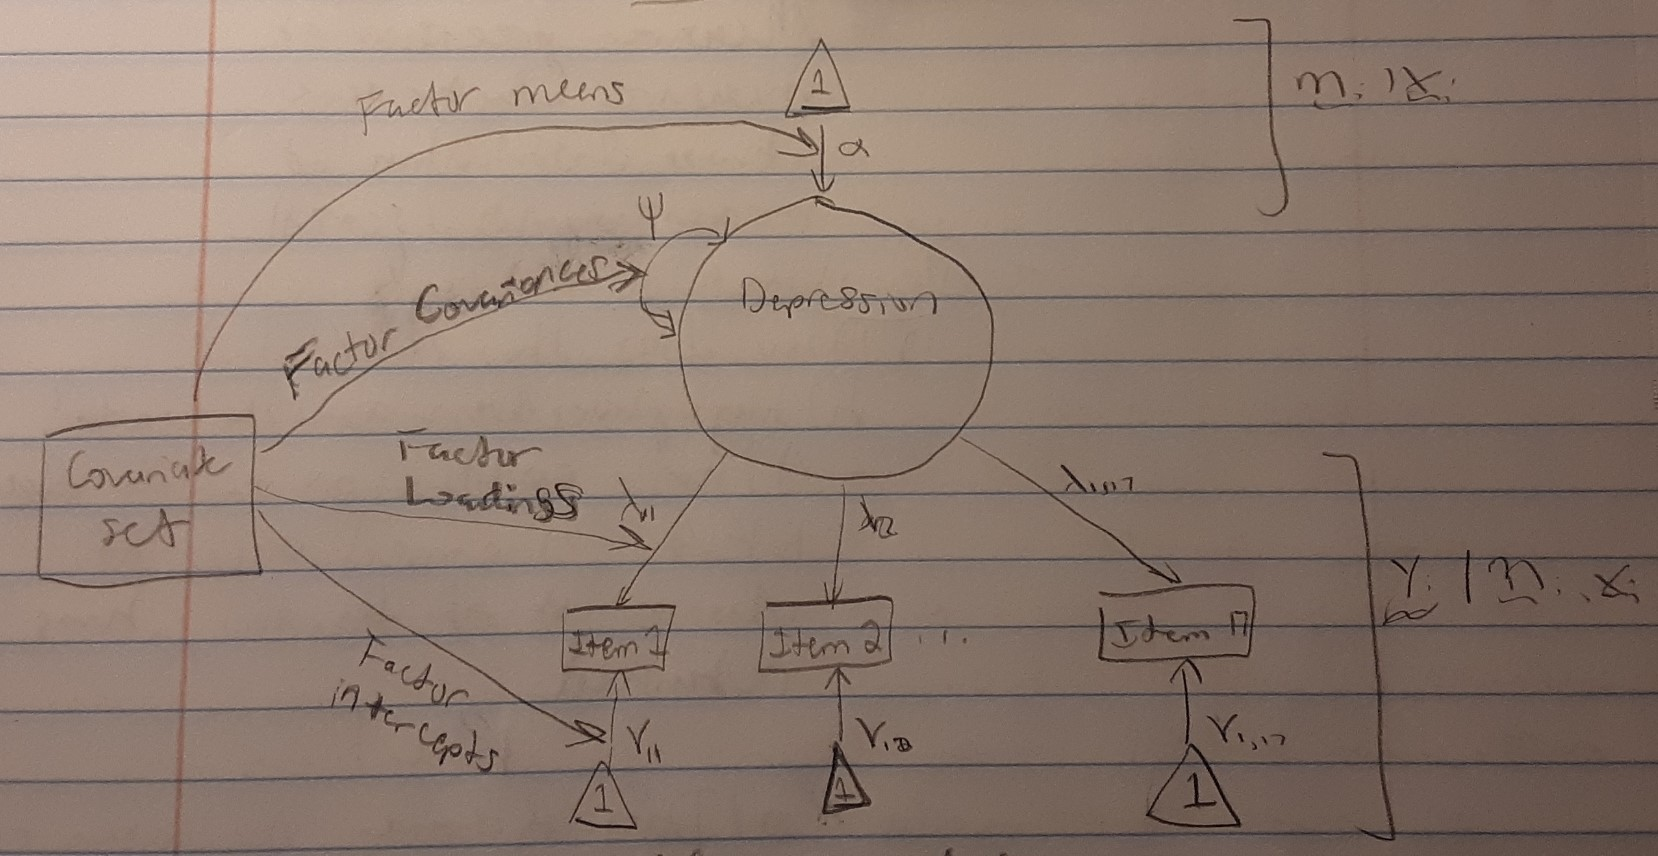
\includegraphics[scale=0.38]{mnlfa_path_diagram.jpg}
\end{center}

\bibliographystyle{plain}
\bibliography{mybib}

\end{document}
